\documentclass[bigger]{beamer}
%\documentclass[handout]{beamer}
\setbeamertemplate{bibliography item}{}
\usepackage[utf8]{inputenc}
\usepackage[english]{babel}
\usepackage{multirow}
\usepackage{synttree}
\usepackage{booktabs}
\usepackage[backend=bibtex,natbib,style=authoryear]{biblatex}
\usetheme{Warsaw}
%\usefonttheme[onlylarge]{structuresmallcapsserif}
\newcommand{\wigegraph}[1]{\begin{figure}[h]
\centering\includegraphics[width=\textwidth]{#1}\end{figure}}
% Ez most valamiert besz.rt, ugyhogy kikommentalom:
%\AtBeginSection[]{\frame{\frametitle{Outline}\tableofcontents[current]}}

\AtBeginPart{\frame{\partpage}} 

\usepackage{tikz}
\usepackage{tikz-qtree}
\usepackage{xspace}

\bibliography{ml}

\newcommand{\defl}{\texttt{dep\_to\_4lang}\xspace}
\newcommand{\difl}{\texttt{dict\_to\_4lang}\xspace}
\newcommand{\tfl}{\texttt{text\_to\_4lang}\xspace}
\newcommand{\tefl}{\texttt{text\_to\_4lang}\xspace}
\newcommand{\fl}{\texttt{4lang}\xspace}

\newcommand{\edge}[3]{\texttt{#1}~$\xrightarrow#2$~\texttt{#3}}
\newcommand{\twoedges}[4]{\texttt{#1}~$\overset{#2}{\underset{#3}{\rightleftharpoons}}$~\texttt{#4}}
\newcommand{\bin}[3]{
    \texttt{#2}~$\xleftarrow1$~\texttt{#1}~$\xrightarrow2$~\texttt{#3}}

\newcommand{\todo}[1]{\textbf{TODO: #1}}

%\usepackage{apacite}
%\let\cite\shortcite  % to get "et al." for more than two authors
%\let\citeA\shortciteA
\begin{document}

\title{Szemantikai elemz\'es gr\'af-transzform\'aci\'okkal}
\author{Kov\'acs \'Ad\'am \\ G\'emes Kinga}
\institute{Automatizálási és Alkalmazott Informatikai Tanszék \\
Budapesti Műszaki és Gazdaságtudományi Egyetem \\
\texttt{adaam.ko@gmail.com}, \texttt{kinga.andrea.gemes@gmail.com}}

\date{Tudományos Diákköri Konferencia\\2018.11.14.}

%-----------------------

\begin{frame} 

\titlepage 

\end{frame} 
%----------------------
\begin{frame}
	\frametitle{M\'ely tanul\'as}
	\begin{itemize}
		\item Elterjedt modell
		\item Term\'eszetes nyelvfeldolgoz\'asban \'elenj\'ar\'o
		\item RNN a sorozatok eset\'en a leghat\'ekonyabb
		\begin{itemize}
			\item LSTM
			\item GRU
		\end{itemize}
	\end{itemize}
\end{frame}
%-----------------------
\begin{frame}
	\frametitle{Yuanfudao rendszer}
	\begin{figure}[h!]
		\centering
		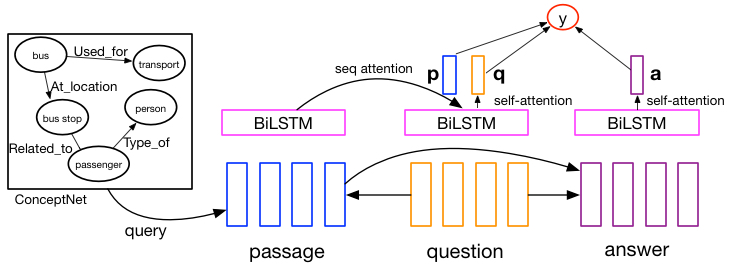
\includegraphics[scale=0.4]{pics/TriAN.jpg}
		\caption{A rendszer strukt\'ur\'aja}
		\label{fig:dnn}
	\end{figure}
\end{frame}
%-----------------------
\begin{frame}
	\frametitle{M\'odos\'it\'asok}
	\begin{itemize}
		\item 4lang hasonl\'os\'ag sz\'am\'it\'as a szavak k\"oz\"ot az el\H{o}feldolgoz\'as sor\'an
		\item \'Uj embedding r\'eteg a 4lang hasonl\'os\'agokhoz
		\item Az RNN r\'eteg b\H{o}v\'it\'ese, hogy a megfelel\H{o} RNN-ek megkapj\'ak a 4lang embedding kimenet\'et
	\end{itemize}
\end{frame}


%-----------------------

\begin{frame}
	\frametitle{Eredm\'enyek}
	\begin{table}[h!]
		\centering
		\begin{tabular}{ | l | c | r | }
			\hline
			modell & dev adat & teszt adat \\ \hline \hline
			el\H{o}tan\'itott TriAN, ConceptNet n\'elk\"ul & 83.7\% & 81.9\% \\ \hline
			el\H{o}tan\'itott TriAN, ConceptNettel & 82.5\% & 80.3\% \\ \hline
			el\H{o}tan\'itott TriAN, 4langgal & 84.2\% & 81.5\% \\ \hline
			\textbf{el\H{o}tan\'itott TriAN, mindkett\H{o}vel} & \textbf{83.4\%} & \textbf{82.9\%} \\ \hline
			TriAN, ConceptNet n\'elk\"ul & 82.8\% & 80.2\% \\ \hline
			TriAN, ConceptNettel & 82.7\% & 80.5\% \\ \hline
			TriAN, 4langgal & 83.2\% & 80.9\% \\ \hline
			TriAN, mindkett\H{o}vel & 83.1\% & 80.8\% \\ \hline
		\end{tabular}
		\caption{A \texttt{4lang} \'es a \texttt{ConceptNet} hat\'asa az eredm\'enyeken}
		\label{tabl:res}
	\end{table}
\end{frame}

%-----------------------
\begin{frame}
    \frametitle{K\"osz\"onj\"uk a figyelmet!}
    \AtNextBibliography{\tiny}
    \printbibliography
\end{frame}
%-----------------------


\end{document}






